\documentclass{standalone}
\usepackage{tikz}
\usepackage{ctex,siunitx}
\setCJKmainfont{Noto Serif CJK SC}
\usepackage{tkz-euclide}
\usepackage{amsmath}
\usetikzlibrary{patterns, calc,3d}
\usetikzlibrary {decorations.pathmorphing,decorations.pathreplacing,decorations.shapes}
\tikzset{label style/.append style={font=\small}}
\begin{document}
\small
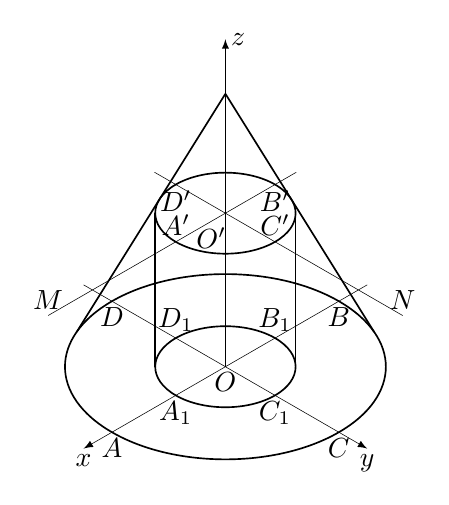
\begin{tikzpicture}[>=latex,scale=1.3,inner sep=2pt,x={(-150:8mm)},z={(-30:8mm)}]
  \draw[very thin,->] (0,0,0)--(0,3.2,0)node[right]{$z$};
\begin{scope}[canvas is xz plane at y=0]
  \draw[very thin,->](-2,0)--(2,0) node[below]{$x$};
  \draw[very thin,->](0,-2)--(0,2) node[below]{$y$};
  \draw[semithick](0,0)circle(0.7)(0,0)circle(1.6);
  \node at (1.6,0) [below] {$A$};
  \node at (-1.6,0) [below] {$B$};
  \node at (0,1.6) [below] {$C$};
  \node at (0,-1.6) [below] {$D$};
  \node at (0.7,0) [below] {$A_1$};
  \node at (-0.7,0) [above] {$B_1$};
  \node at (0,0.7) [below] {$C_1$};
  \node at (0,-0.7) [above] {$D_1$};
  \node at (0,0) [below] {$O$};
\end{scope}
\begin{scope}[canvas is xz plane at y=1.5]
  \draw[very thin](-1,0)--(2.5,0)node[above]{$M$};
  \draw[very thin](0,-1)--(0,2.5)node[above]{$N$};
  \draw[semithick](0,0)circle(0.7);
  \node at (0.7,0) [above] {$A'$};
  \node at (-0.7,0) [below] {$B'$};
  \node at (0,0.7) [above] {$C'$};
  \node at (0,-0.7) [below] {$D'$};
  \node at (0.2,0) [below] {$O'$};
\end{scope}
\draw[semithick]({0.7*cos(-45)},0,{0.7*sin(-45)})--({0.7*cos(-45)},1.5,{0.7*sin(-45)});
\draw[semithick]({0.7*cos(135)},0,{0.7*sin(135)})--({0.7*cos(135)},1.5,{0.7*sin(135)});
\draw[semithick](0,8/3,0)--({1.6*cos(-67)},0,{1.6*sin(-67)});
\draw[semithick](0,8/3,0)--({1.6*cos(157)},0,{1.6*sin(157)});
\end{tikzpicture}
\end{document}